% Preamble. Don't worry about it.
\documentclass{article}
\usepackage{setspace,graphicx}
\usepackage[utf8]{inputenc}
\usepackage[left=1in,top=1in,right=1in,bottom=1in]{geometry} % Document margins
\onehalfspacing

% Setting the depth for Table of Contents
\setcounter{tocdepth}{1}

\begin{document}

% --- TITLE PAGE ---
\title{Donnervögel Consulting \\ Streamlined Grading System}
\author{\textbf{Phase Lead: Ian Pun} \\ Markus Balaski \\ Stephen Laboucane \\
  Graeme Smith \\ Jordan Toering \\  Colin Woodbury \\ Chazz Young}
\date{\today}
\maketitle
\clearpage
% ------------------

% --- REVISION HISTORY ---
\textbf{Revision History}
\begin{center}
  \begin{tabular}{| c | c | c | l |}
    \hline
    Version & Date & Members & Changes\\
    \hline
    1.0 & 2014 Mar 07 (Fri) & Markus B. & Document created\\
    & & Graeme S. & \\
    & & Jordan T. & \\
    & & Stephen L. & \\
    & & Ian P. & \\
    & & Colin W. & \\
    & & Chazz Y. & \\
    \hline
  \end{tabular}
\end{center}
\clearpage
% ------------------------

% --- TABLE OF CONTENTS ---
\tableofcontents
\clearpage
% -------------------------

% ---
\section{Product Overview}  % 5 Marks
% THIS SHOULD BE 1/2 TO 1 PAGE IN LENGTH!
% Markus will do this.

% ---
\section{Getting Started}
\emph{No contents here.}

\subsection{Software Requirements}

\subsection{Hardware Requirements}

\subsection{Installation}

\subsection{Running the Application}

\subsection{UAT??}

% ---
\section{Functions and User Interface Description}  % 30 Marks total
% This is a very big section.
% 1. How is a function selected?
% 2. How is input entered? (Include pictures)
% 3. What keys need to be pressed?
% 4. What will the user see when a step is performed correctly?
% 5. What will the user see when a step is performed incorrectly? (errors)
\subsection{Login}

\subsection{Landing Page}
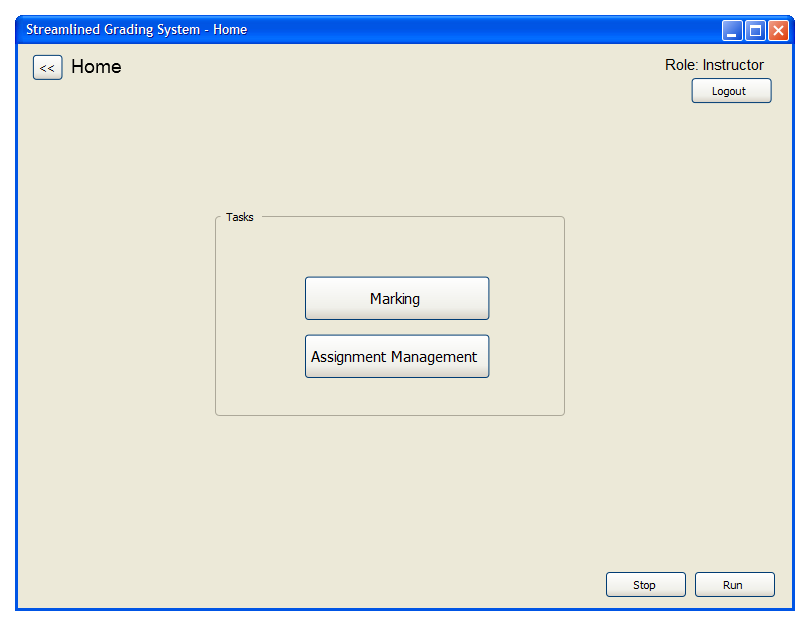
\includegraphics[scale=0.6]{../images/UIMockups/PNG_Renders/LandingPage}
The Landing Page is shown to all users of the system following login.  The Tasks box shows actions that each user can do.  It does not show actions the user cannot do.

\subsection{System Admin Panel}

\subsection{Database Panel}

\subsection{User Account Panel}

\subsection{System Panel}

\subsection{Manage Courses}

\subsection{Modify Courses}

\subsection{Choose Course}

\subsection{Choose Activity}

\subsection{Modify Activity}

\subsection{Copy Activty}

\subsection{Modify Rubric}

\subsection{Select Activity}

\subsection{Test Suite}
\begin{center}
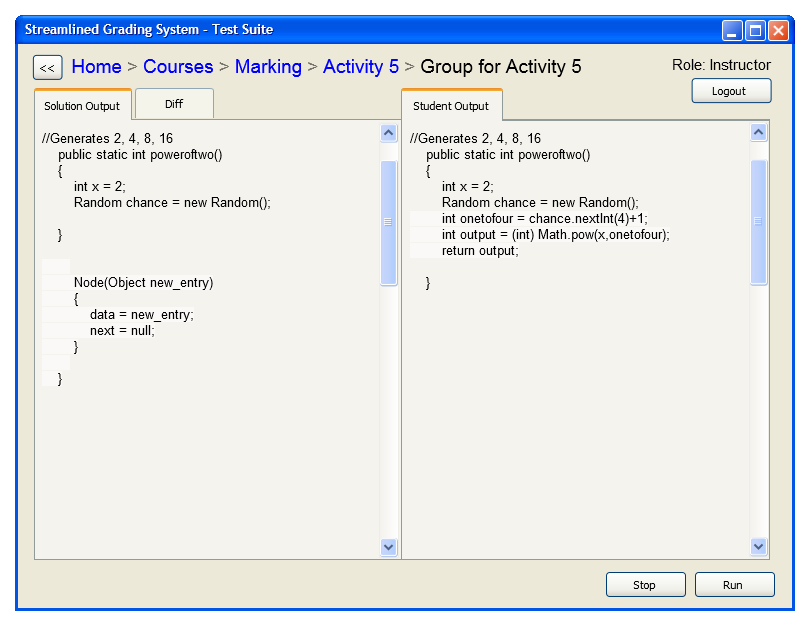
\includegraphics[scale=0.6]{../images/UIMockups/PNG_Renders/SRS_TestSuite_Split}
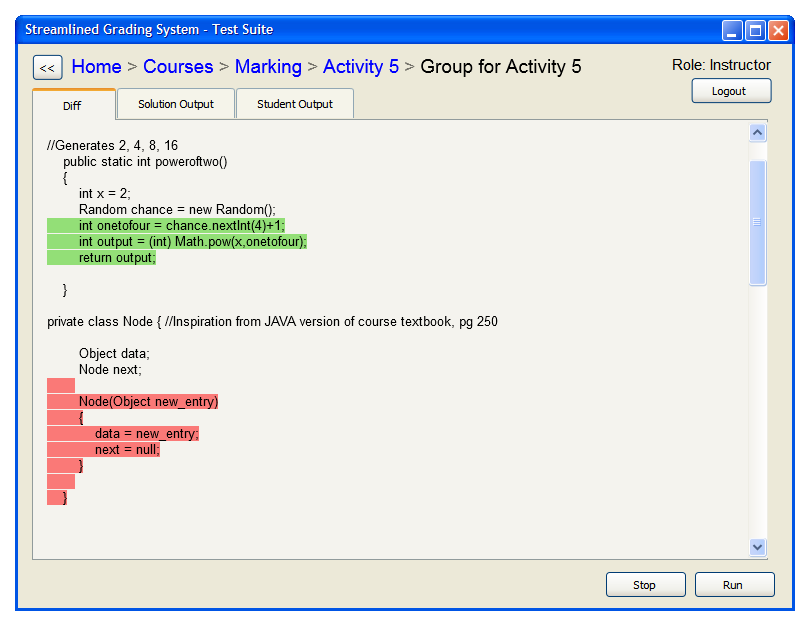
\includegraphics[scale=0.6]{../images/UIMockups/PNG_Renders/SRS_TestSuite_Tabs}
\end{center}

\subsection{Assignment Page}

% ---
\section{Quick Reference}  % 9 Marks

% ---
\section{Known Bugs}
There are no bugs, our software is perfect.

\end{document}
